\ifspanish

\question 
La región sombreada de la figura ilustra el dominio de la función de distribución conjunta de $S$ y $X$, i.e., el conjunto de puntos para los que $p_{X,S}(x,s)\neq 0$.

\vspace{.3cm}
\centerline{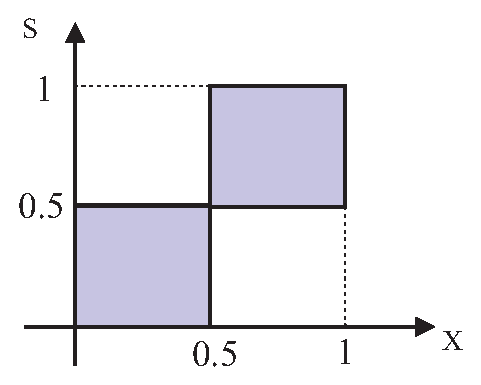
\epsfig{file=Figuras/graph_pxs,width=6cm}}
\vspace{.3cm}

Responda a las siguientes cuestiones \underline{justificando} sus respuestas:

\begin{parts}
\part Si se sabe que $p_{X,S}(x,s)$ es constante en el dominio de definición, ¿cuál es el estimador MSE de $S$ a la vista de $X$? Represente gráficamente dicho estimador.
\part ¿Existe alguna $p_{X,S}(x,s)$ con el dominio anterior para la cual el estimador MSE de $S$ a la vista de $X$ sea $\widehat S_{\text{MSE}} = X/2$?
\part Justifique si existe alguna $p_{X,S}(x,s)$ con el dominio anterior tal que $\widehat S = 0.5$ sea:
\begin{itemize}
\item El estimador de mínimo error cuadrático de $S$ a la vista de $X$.
\item El estimador de mínimo error absoluto de $S$ a la vista de $X$.
\item El estimador de máximo a posteriori de $S$ a la vista de $X$.
\end{itemize}
\end{parts}

\begin{solution}
  \begin{parts}
\part $\widehat S_{\text{MSE}} = 0.25$ si $0<x<0.5$ y $\widehat S_{\text{MSE}} = 0.75$ si $0.5<x<1$ 

\part Para $0.5<x<1$, $p _{S|X}(s|x)$ está definida entre $0.5<s<1$, por lo que $X/2$ no puede ser el valor medio de $p _{S|X}(s|x)$
  
 \part   $\widehat S = 0.5$ no puede ser ni la media ni la mediana de $p_{S|X}(s|x)$, pero puede ser su máximo.  Luego, $\widehat S = 0.5$  no puede ser ni $\widehat S_{\text{MSE}} $, ni  $\widehat S_{\text{MAD}} $, pero puede ser  $\widehat S_{\text{MAP}} $.
 \end{parts}
 \end{solution}

\else

\question 
In the plot below, the shaded region shows the domain of a joint distribution of $S$ and $X$, i.e., the set of points for which $p_{X,S}(x,s)\neq 0$.

\vspace{.3cm}
\centerline{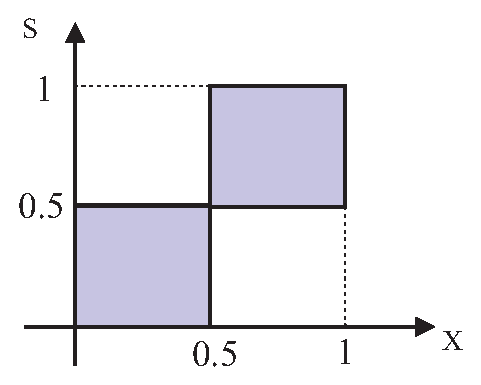
\epsfig{file=Figuras/graph_pxs,width=6cm}}
\vspace{.3cm}

Please, provide \underline{justified} answers to the following questions:

\begin{parts}
\part If it is known that $p_{X,S}(x,s)$ is constant in its domain, which is the MSE estimator of $S$ given $X$? Provide a graphical representation of this estimator.
\part Is there any $p_{X,S}(x,s)$ with the previous domain for which the MSE estimator of $S$ given $X$ is $\widehat S_{\text{MMSE}} = X/2$?
\part Justify if there exists any $p_{X,S}(x,s)$ with the previous domain, so that $\widehat S = 0.5$ is:
\begin{itemize}
\item The minimum mean square error estimator of $S$ given $X$.
\item The minimum mean absolute deviation estimator of $S$ given $X$.
\item The maximum {\em a posteriori} estimator of $S$ given $X$.
\end{itemize}
\end{parts}

\begin{solution}
  \begin{parts}
\part $\widehat S_{\text{MMSE}} = 0.25$ for $0<x<0.5$ and $\widehat S_{\text{MMSE}} = 0.75$ for $0.5<x<1$ 

\part When $0.5<x<1$, $p _{S|X}(s|x)$ is non-zero for $0.5<s<1$, thus $X/2$ can never be the mean of $p _{S|X}(s|x)$ for that range of $X$.
  
 \part   $\widehat S = 0.5$ cannot be the mean or the median of $p_{S|X}(s|x)$, but it can be its maximum.  Therefore, $\widehat S = 0.5$  can just be  $\widehat S_{\text{MAP}} $ (but not  $\widehat S_{\text{MMSE}} $ or $\widehat S_{\text{MAD}} $).
 \end{parts}
 \end{solution}

\fi